\newenvironment{mytest}[4]
{
    \begin{center}
        \centering
        \begin{tabular}[h]{|m{4cm}|m{12cm}|}
            \hline
            \rowcolor[HTML]{F8B400}
            \textbf{But}    & #1 \\
            \hline
            \hline
            \rowcolor[HTML]{F7F7F7}
            Entrée          & #2 \\
            \hline
            \rowcolor[HTML]{F7F7F7}
            Scénario        & #3 \\
            \hline
            \rowcolor[HTML]{F7F7F7}
            Analyse du test & #4 \\
            \hline
        \end{tabular}
    \end{center}
}

\section{Nos tests}
Nous avons mis en place divers outils pour contrôler notre implémentation :
\begin{itemize}
    \item Chaque {\tt commit} sera vérifier par des pipelines de {\tt GitLab}. Cet outil compile le code proposé sur une machine afin de voir si le code suggérer n'a aucune erreur de compilation.
    \item L'implémentation de notre {\tt backend} est contrôlé par le framework {\tt NYC}. Nos tests sont surveillés par le framework et nous donne le résultat de {\tt coverage} pour chaque fichier testé.
\end{itemize}

\subsection{Test unitaire}

Consigne : description des tests, discussion de leurs résultats, explication des problèmes, des défauts et bugs. Pour chacun des tests avec : (1) spécification et buts du test ;
(2) cas de tests (données) utilisé ; (3) scénario du test ; (4) analyse du test et les moyens de mise en œuvre de cette analyse.

\subsubsection{Vérification des fichiers dans le fichier {\tt src}}

\mytest
{Vérifier si les fichiers possède le bon format (\texttt{.ts}) dans le dossier \texttt{src/main}}
{Un ensemble de fichiers}
{En cas de mauvais format dans le dossier, on affiche les fichiers qui ne respectent pas le format \texttt{.ts}}
{Parcours d'un dossier en ajoutant dans une liste les fichiers qui ne respecte pas la condition}

\mytest
{Vérifier si les fichiers possède le bon format (\texttt{.ts} ou \texttt{.json}) dans le dossier \texttt{src/test}}
{Un ensemble de fichiers}
{En cas de mauvais format dans le dossier, on affiche les fichiers qui ne respectent pas le format \texttt{.ts} ou \texttt{.json}}
{Parcours d'un dossier en ajoutant dans une liste les fichiers qui ne respecte pas la condition}

\mytest
{Chaque fichier possède une classe doit commencer par une majuscule dans le dossier \texttt{src/main}}
{Un ensemble de fichiers}
{En cas de non-respect des consignes, on affiche les fichiers qui ne respectent la capitalisation de la première lettre}
{On ajoute dans une liste les fichiers qui ne respecte pas la condition (parcours d'un dossier + manipulation de chaîne de caractère pour récupérer la première}

\subsubsection{Vérification de la carte du jeu}

\mytest
{Vérification de l'emplacement d'une case d'hexagone \#1}
{Identifiant d'une vraie case d'hexagone}
{Si l'identifiant n'est pas sur la carte du jeu, signalez cette case}
{Vérifie l'identifiant dans une table de hachage}

\mytest
{Vérification de l'emplacement d'une case d'hexagone \#2}
{Identifiant d'une fausse case d'hexagone}
{Si l'identifiant est inclus sur la carte du jeu, signalez cette case}
{Vérifie l'identifiant dans une table de hachage}

\subsubsection{Vérification du serveur {\tt socket}}

\mytest
{Vérification si le port du client est stocké correctement}
{Un entier représentant le port du client}
{En cas d'une inégalité entre le port du client et le port enregistré pour le serveur socket, nous levons une exception}
{On vérifie avec une comparaison entre deux entiers}

\mytest
{Vérification si le port du serveur est stocké correctement}
{Un entier représentant le port du serveur}
{En cas d'une inégalité entre le port du serveur et le port enregistré pour le serveur socket, nous levons une exception}
{On vérifie avec une comparaison entre deux entiers}

\mytest
{Vérification de la limite de joueurs dans une partie (2 joueurs maximum)}
{La connexion d'un joueur}
{En cas de connexion d'un troisième joueur, une exception est levée}
{Avant de vérifier la connexion d'un troisième joueur, nous attendons 500 millisecondes}

\mytest
{Vérification du lancement de la partie}
{Une instance du \texttt{serveur}}
{Avec notre instance du serveur, on essaye de récupérer le jeu, si ce n'est pas le cas, on lève une exception}
{On vérifie l'instance du jeu avec l'instance du serveur}

\mytest
{Vérification du joueur \#1 dans la partie}
{Une instance du \texttt{serveur}}
{Si le joueur \#1 n'est pas accessible via l'instance du jeu, nous levons une exception}
{On vérifie dans l'instance du jeu qui est accessible à partir de l'instance du serveur}

\mytest
{Vérification du joueur \#2 dans la partie}
{Une instance du \texttt{serveur}}
{Si le joueur \#2 n'est pas accessible via l'instance du jeu, nous levons une exception}
{On vérifie dans l'instance du jeu qui est accessible à partir de l'instance du serveur}

\mytest
{Vérification de l'identifiant du socket du joueur \#1}
{Une instance du \texttt{serveur}}
{
    \begin{itemize}
        \item Le joueur \#1 possède le socket du joueur \#2 $\rightarrow$ exception
        \item Le jeu ne possède pas le bon identifiant du joueur \#1 $\rightarrow$ exception
    \end{itemize}
}
{On récupère les identifiants des différents joueurs dans l'instance du jeu (accessible à partir de l'instance du serveur)}

\mytest
{Vérification de l'identifiant du socket du joueur \#2}
{Une instance du \texttt{serveur}}
{
    \begin{itemize}
        \item Le joueur \#2 possède le socket du joueur \#1 $\rightarrow$ exception
        \item Le jeu ne possède pas le bon identifiant du joueur \#2 $\rightarrow$ exception
    \end{itemize}
}
{On récupère les identifiants des différents joueurs dans l'instance du jeu (accessible à partir de l'instance du serveur)}

\mytest
{Vérification de la fin de partie lors de la déconnexion d'un joueur}
{Une instance du serveur et le socket d'un joueur}
{Si le jeu est accessible à partir du joueur déconnecté, alors nous levons une exception}
{On vérifie dans l'instance du serveur, si on peut récupérer le jeu}

\mytest
{Vérifier si le dernier joueur reste connecté au jeu malgré la déconnexion de son adversaire}
{Une instance du \texttt{serveur}}
{On doit retrouver un joueur dans l'instance du \texttt{serveur}, sinon on lève une exception}
{
    \begin{itemize}
        \item On vérifie la longueur de la liste des joueurs
        \item Le dernier joueur possède le bon identifiant
        \item On vérifie si le joueur a bien été supprimé de la liste des joueurs
    \end{itemize}
}

\mytest
{Vérification du redémarrage du jeu lors de la connexion du premier joueur}
{Socket du premier joueur et une instance du \texttt{serveur}}
{Si le joueur ne reçoit pas une instance du jeu, nous levons une exception}
{Lors de la connexion du joueur, il reçoit le jeu}

\mytest
{Vérification du redémarrage du jeu lors de la connexion du deuxième joueur}
{Socket du deuxième joueur et une instance du \texttt{serveur}}
{Si le joueur ne reçoit pas une instance du jeu, nous levons une exception}
{Lors de la connexion du joueur, il reçoit le jeu}

\mytest
{Vérification de la communication entre le serveur et le client (joueur)}
{Le socket d'un joueur}
{Le joueur envoie un message \texttt{ping} au serveur. Il sera immédiatement répondu par le serveur par un message \texttt{pong}}
{Le client envoie un message et attends une réponse du serveur.}

\mytest
{Vérification de la communication entre le serveur et le client}
{Les sockets des deux joueurs}
{On vérifie si un message part du point A au point B, sinon on lève une exception}
{Le joueur \#1 envoie un message \quotes{\texttt{Hello world}} et on vérifie si le joueur \#2 a reçu le message}

\subsubsection{Vérification de la machine d'état}
\mytest
{Vérification de l'instanciation de la machine d'état}
{Les spécificités nécessaires pour démarrer la machine d'état, dont les phases}
{Nous affichons une erreur si la machine n'est pas bien instanciée}
{Vérifie si l'état actuel est l'état initial}

\mytest
{Vérification du redémarrage de la machine d'état}
{La machine d'état lancée dans le test précédent}
{Nous affichons une erreur incluant l'état actuel et l'état attendu si la machine n'est pas bien redémarrée}
{Vérifie si l'état actuel est bien l'état initial}

\mytest
{Vérification des transitions de la machine d'état}
{La machine d'état lancée dans le premier test de cette section}
{Nous affichons une erreur incluant l'état actuel et l'état attendu si l'état n'est pas bien changé}
{Vérifie après chaque appel au changement de l'état actuel de la machine d'état si ce dernier est correct}

\mytest
{Vérification du compteur de tours}
{La machine d'état lancée dans le premier test de cette section}
{Nous affichons une erreur incluant l'état actuel et l'état attendu si l'état actuel est erroné}
{Vérifie si après une série de changements de phases, la machine d'état met bien à jour le nombre du tour actuel}

\mytest
{Vérification du compteur de tours}
{La machine d'état lancée dans le premier test de cette section}
{Nous affichons une erreur incluant le nombre de tours actuels et le nombre de tours attendu si le nombre de tours est incorrect}
{Vérifie si après une série de changements de phases, la machine d'état met bien à jour le nombre du tour actuel}

\mytest
{Vérification le changement de phases pendant un tour}
{La machine d'état lancée dans le premier test de cette section}
{Nous affichons une erreur incluant l'état actuel et l'état attendu si l'état actuel est erroné}
{Vérifie si après une série de changements de phases égale au nombre totale de phases dans le jeu, l'état de la machine d'état est initiale}

\subsubsection{Vérification de l'instance du jeu}

\mytest
{Vérification de l'instantiation du serveur du jeu}
{L'adresse du client, le port du serveur et l'instance de la machine d'état}
{Nous affichons une erreur si l'instance du jeu n'est pas bien instanciée}
{Vérifie si le serveur du jeu se lance sans erreurs}

\mytest
{Vérification de l'instanciation du joueur 1}
{Le port du serveur pour que nous puisions connecter le premier joueur}
{Nous affichons une erreur si le premier joueur n'est pas bien connecté}
{Vérifie si le premier joueur se connecte sans erreur}

\mytest
{Vérification de l'instanciation du joueur 2}
{Le port du serveur pour que nous puisions connecter le deuxième joueur}
{Nous affichons une erreur si le deuxième joueur n'est pas bien connecté}
{Vérifie si le deuxième joueur se connecte sans erreur}

\mytest
{Vérification du lancement du jeu}
{Le serveur du jeu}
{Nous affichons une erreur si le jeu n'est pas bien lancé, ainsi que si les deux joueurs sont bien connectés ou pas}
{Vérifie si le jeu se lance sans erreur après la connexion des 2 joueurs}

\mytest
{Vérification de la commande {\tt units} tant que premier joueur}
{La {\tt socket} du premier joueur}
{Nous affichons une erreur si le premier joueur n'a pas reçu le bon résultat en exécutant la commande {\tt units} ainsi que le nombre correct et actuel si ce dernier est incorrect}
{Vérifie si le premier joueur reçoit bien ses unités avec leurs spécificités après l'appel à la commande {\tt units}}

\mytest
{Vérification de la commande {\tt units} tant que deuxième joueur}
{La {\tt socket} du deuxième joueur}
{Nous affichons une erreur si le deuxième joueur n'a pas reçu le bon résultat en exécutant la commande {\tt units} ainsi que le nombre correct et actuel si ce dernier est incorrect}
{Vérifie si le deuxième joueur reçoit bien ses unités avec leurs spécificités après l'appel à la commande {\tt units}}

\mytest
{Vérification de la commande {\tt move} tant que premier joueur avec des arguments corrects}
{La {\tt socket} du premier joueur, ainsi que les arguments corrects pour la commande {\tt move}}
{Nous affichons une erreur si le premier joueur n'a pas bien effectué {\tt move} ainsi que l'erreur correspondante}
{Vérifie si le premier joueur effectue correctement le mouvement après l'appel à la commande {\tt move} avec des arguments valides}

\mytest
{Vérification de la commande {\tt move} tant que premier joueur avec des arguments incorrects, dont un identifiant d'unité incorrect}
{La {\tt socket} du premier joueur, ainsi qu'une unité incorrecte comme argument pour la commande {\tt move}}
{Nous affichons une erreur si le premier joueur a pu effectuer la commande {\tt move} avec une unité qu'il ne peut pas bouger}
{Vérifie si le premier joueur ne peut pas effectuer le mouvement après l'appel à la commande {\tt move} avec une unité incorrecte comme argument}

\mytest
{Vérification de la commande {\tt move} tant que premier joueur avec des arguments incorrects, dont un identifiant d'hexagone incorrect}
{La {\tt socket} du premier joueur, ainsi qu'un identifiant d'hexagone incorrect pour la commande {\tt move}}
{Nous affichons une erreur si le premier joueur a pu effectuer la commande {\tt move} avec un identifiant d'hexagone qui n'existe pas}
{Vérifie si le premier joueur ne peut pas effectuer le mouvement après l'appel à la commande {\tt move} avec un identifiant d'hexagone incorrect comme argument}

\mytest
{Vérification de la commande {\tt move} tant que premier joueur avec des arguments incorrects, dont l'identifiant d'une unité de l'adversaire}
{La {\tt socket} du premier joueur, ainsi qu'un identifiant d'unité adversaire pour la commande {\tt move} du premier joueur}
{Nous affichons une erreur si le premier joueur a pu effectuer la commande {\tt move} avec un identifiant d'unité de l'adversaire}
{Vérifie si le premier joueur ne peut pas effectuer le mouvement après l'appel à la commande {\tt move} avec un identifiant d'unité de l'adversaire comme argument}

\mytest
{Vérification de la commande {\tt move} tant que deuxième joueur avec des arguments corrects}
{La {\tt socket} du deuxième joueur, ainsi que les arguments corrects pour la commande {\tt move}}
{Nous affichons une erreur si le deuxième joueur n'a pas bien effectué {\tt move} ainsi que l'erreur correspondante}
{Vérifie si le deuxième joueur effectue correctement le mouvement après l'appel à la commande {\tt move} avec des arguments valides}

Nous n'avons pas testé les mêmes commandes que le premier joueur car elles sont similaires à celles du premier joueur



\subsubsection{Vérification de joueur}

\mytest
{Vérification de la création du joueur }
{Un  {\tt joueur} avec en paramètre un identifiant et un socket}
{Si le joueur n'a pas d'id et/ou de base et/ou Unités d'approvisionnement, signalez cette erreur}
{Vérifie l'appel d'un {\tt joueur}}


\mytest
{Vérification d'ajout d'Unités }
{Un {\tt joueur} et une {\tt unité}}
{S'il n'y a pas d'Unités ou si l'unité est incorrect, signalez cette case, sinon l'ajouter}
{Vérifie l'ajout d'unité}


\mytest
{Vérification de l'ajout et de la suppression du Dump }
{Un nouveau {\tt joueur} avec en paramètre un identifiant et un socket et un {\tt Dump} avec les arguments correcte}
{Si l'identifiant est inclus sur la carte du jeu, signalez cette case}
{Vérifie l'ajout et la suppression du Dump}


\subsubsection{Vérification de la classe abstraite {\tt Player}}

\mytest
{Vérification de l'initialisation de l'unité}
{Une instance de l'unité}
{Si l'instance de l'unité ne contient pas les mêmes valeurs données lors de sa création, alors on lève une exception}
{On vérifie dans chaque attribut de l'unité, si l'initialisation est correcte}

\mytest
{Vérification de la valeur du retour du jeu de dé}
{Un dé}
{Si le dé ne sort pas une valeur entre \texttt{1} et \texttt{6}, alors on lève une exception}
{On lance un dé, et on regarde sa valeur}

\mytest
{Vérification de l'exportation d'une unité en format \texttt{json}}
{Une instance du joueur et son unité}
{On vérifie si ces valeurs initiales sont correctes, sinon on lève une exception}
{
    On regarde plusieurs de ces attributs :
    \begin{itemize}
        \item Son identifiant
        \item Sa position
        \item Ses points de mouvements
        \item Son type
        \item Son propriétaire
    \end{itemize}
}

\mytest
{Vérification de l'ajout et de la suppression des unités}
{Une instance du joueur et son unité}
{On vérifie les changements effectuer par l'ajout et la suppression des unités}
{On observe combien d'unités possède le joueur}

\mytest
{Vérification de la perte de vie pour une unité}
{Une instance d'une unité}
{Si l'unité contient une valeur négative pour ces points de vie, on lève une exception}
{Nous regardons directement dans ces points de vie}

\subsubsection{Vérification des bases}

\mytest
{Vérification de l'appel d'une Base}
{Une nouvelle {\tt Base} avec en paramètre un {\tt HexID}, une primary et son identifiant }
{Si la Base n'a pas le bon id et/ou n'a pas la bonne position et/ou si ce n'est pas primaire, signaler l'erreur }
{Vérifie le bon appel d'une base}

\mytest
{Vérification qu'une base envoie correctement}
{Une base}
{Si la base ne peut pas envoyer,  signaler l'erreur }
{Vérifie le bon envoie de la base }

\mytest
{Vérification qu'une base reçoit correctement}
{Une base}
{Si la base ne peut pas recevoir,  signaler l'erreur }
{Vérifie le bon envoie de la base }

\mytest
{Vérification qu'une base réinitialise correctement}
{Une base}
{Si la base ne peut pas envoyer et/ou recevoir,  signaler l'erreur }
{Vérifie la bonne initiation de la base }

\mytest
{Vérification qu'une base place correctement}
{Une base et un nouveau {\tt HexID}}
{Si la base a la même position qu'au début,  signaler l'erreur }
{Vérifie le bon placement fait par la  base }

\subsubsection{Vérification de l'attaque}

\mytest
{Vérifier si le combat retourne les bons résultats de dégâts et applique les bons effets}
{Une unité attaquante et une unité défenseuse}
{Si un résultat doit détruire une unité ou au contraire ne rien faire, les effets se répercutent dans le jeu}
{Nous vérifions pour les résultats aléatoires possibles, tout résultat de combat est bien appliqué. Notamment vérifier
    qu'une unité est bien détruite, si elle perd les bons points de vie ou si elle est toujours vivante}

\mytest
{Vérifier si le combat retourne les bons résultats de morale et applique les bons effets}
{Une unité attaquante et une unité défenseuse}
{Si un résultat doit forcer une unité à se replier ou non, alors le changement doit être visible dans le jeu}
{Nous vérifions pour les résultats aléatoires possibles, que si une unité doit se replier, alors l'unité se
    déplace loin de l'ennemie. S'il ne faut pas alors elle doit rester au même endroit.}

\subsubsection{Vérification du combat}

\mytest
{Vérifier si le simulateur de combat retourne les bons résultats pour les dégâts}
{Un nombre d'attaquants et de défenseurs, un entier représentant le moral et un type de terrain}
{Chaque combinaison de paramètres doit retourner le même résultat exact à chaque fois}
{Nous prenons quatre combinaisons d'entrées distinctes.
    En divisant le nombre d'attaquants par le nombre de défenseurs, on applique les règles du jeu pour définir
    quelle case du tableau des résultats de combat, il faut obtenir. Pour ne pas avoir des résultats aléatoires comme
    il le faut normalement et avoir des tests exacts, nous ne lancons pas de dé.}

\mytest
{Vérifier si le simulateur de combat retourne les bons résultats pour le moral}
{Un nombre d'attaquants et de défenseurs, un entier représentant le moral et un type de terrain}
{Chaque combinaison de paramètres doit retourner le même résultat exact à chaque fois}
{Nous prenons les quatre combinaisons d'entrées distinctes.
    En divisant le nombre d'attaquants par le nombre de défenseurs, on applique les règles du jeu pour définir
    quelle case du tableau des résultats de combat, il faut obtenir. Pour ne pas avoir des résultats aléatoires comme
    il le faut normalement et avoir des tests exacts, nous ne lançons pas de dé.}


\subsubsection{Vérification du jeu}

\mytest
{Vérification de l'initialisation du jeu}
{Une instance du jeu}
{Le jeu doit s'initialiser correction, sinon on lève une exception}
{On observe la valeur de retour de l'instance du jeu}

\mytest
{Vérification des unités qui peuvent se déplacer}
{Un joueur}
{Les unités qui sont capables de bouger doivent être présentes dans la liste}
{En étant au début du jeu, toutes les unités doivent être capables de bouger. Nous vérifions donc si elles sont toutes présentes dans la liste retournée}

\mytest
{Vérification de l'approvisionnement d'une unité}
{Un joueur, une liste d'unités, une liste de bases et dump, ainsi qu'une liste d'unité de soutien}
{Vérifier si il existe un chemin entre une unité et une base ou un dump proche. Si c'est pas le cas, étendre le chemin avec les unités de soutien. Si il n'y a toujours pas de
chemin, alors lever une exception}
{Pour toutes les unités du joueur, dans l'état initial du jeu, il faut qu'elles ont toutes accés a l'approvisionnement, comme les conditions sont satisfaites}

\mytest
{Vérification de l'embarcation dans une unité de soutien}
{Une unité de soutien, un dump et un joueur}
{Si le dump n'est pas dans les objets embarqués de l'unité après avoir été embarqué, lever une exception}
{Il faut tout d'abord bouger l'unité de soutien à la position du dump et l'embarquer dans l'unité. Puis nous essayons d'embarquer le dump dans celle ci. Si tout se
passe bien, alors le dump devrait être visible dans les objets que l'unité de soutien a dejà embarquée}

\mytest
{Vérification du débarquement}
{Un joueur et une unité de soutien}
{L'unité de soutien doit désembarquer l'objet qu'elle porte. Si elle ne portait rien ou si l'objet est toujours embarqué ou si l'objet n'est pas visible sur la carte, lever
une exception}
{Pour une unité de soutien donnée, nous savons qu'elle porte sur elle un dump. En le déposant, il doit maintenant être visible dans l'hexagone dans lequel nous l'avons
posé, et que l'unité de soutien n'ai pas d'autres objets portés}

\subsubsection{Vérification de la recherche du plus court chemin}

\mytest
{Vérifier si le chemin renvoyé est le plus court}
{Identifiant d'un hexagone de départ, l'identifiant d'un hexagone de destination et l'unité qui se déplace}
{Pour un hexagone de départ et de destination donné, un plus court chemin a toujours le même poids. Nous vérifions
    s'il est égale à celui ci}
{En ayant une unité qui est adjacente à une unité ennemie, nous vérifions si le calcul de cout est correcte, car
    le plus court chemin passe à côté d'elle, ce qui teste plusieurs scenarios qui peuvent être rencontrés dans le jeu}

\mytest
{Vérifier si une unité ne passe pas par un hexagone qui contient des ennemis}
{Identifiant d'un hexagone de départ, l'identifiant d'un hexagone de destination et l'unité qui se déplace}
{Si on trouve un plus court chemin entre deux hexagones, le chemin ne doit pas contenir un hexagone qui a des
    unités ennemies.}
{En prenant un plus court chemin, nous vérifions pour tous les hexagones du chemin, s'il n'appartient pas
    au joueur qui tente de bouger l'unité.}

\subsection{Couverture du code}

Le framework {\tt nyc} nous permet de tester la couverture. Il faut lancer la commande {\tt yarn test} dans le \lstinline{backend} ce qui créé dans le dossier \lstinline{coverage} où se trouve à l'intérieur un \lstinline{index.html} qui donne ceci.

\begin{figure}[H]
    \centering
    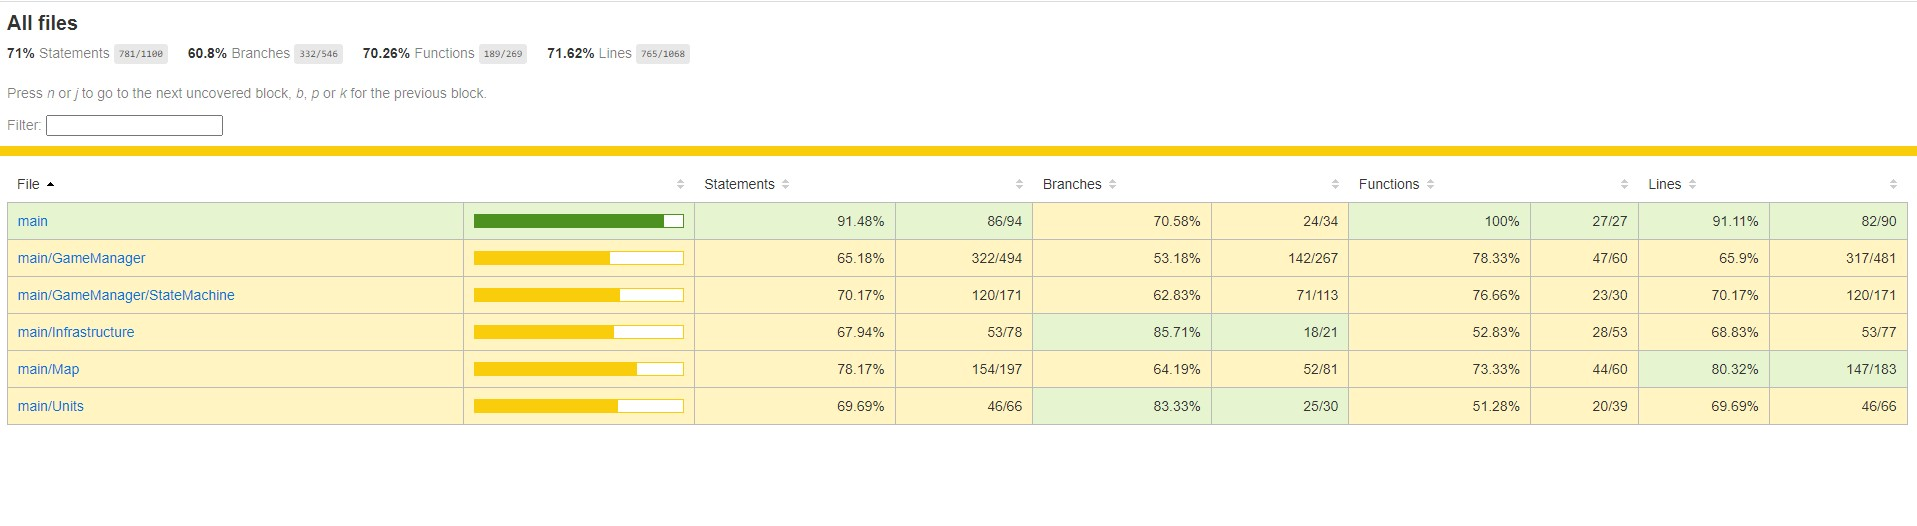
\includegraphics[scale=0.35]{data/couverture_test_1.jpg}
    \caption{Couverture générale du backend}
\end{figure}

On peut voir le pourcentage de couverture de chaque fichier. On peut aussi aller plus dans les détails et regarder ligne par ligne pour être sûr qu'absolument tout le code soit testé.

\begin{figure}[H]
    \centering
    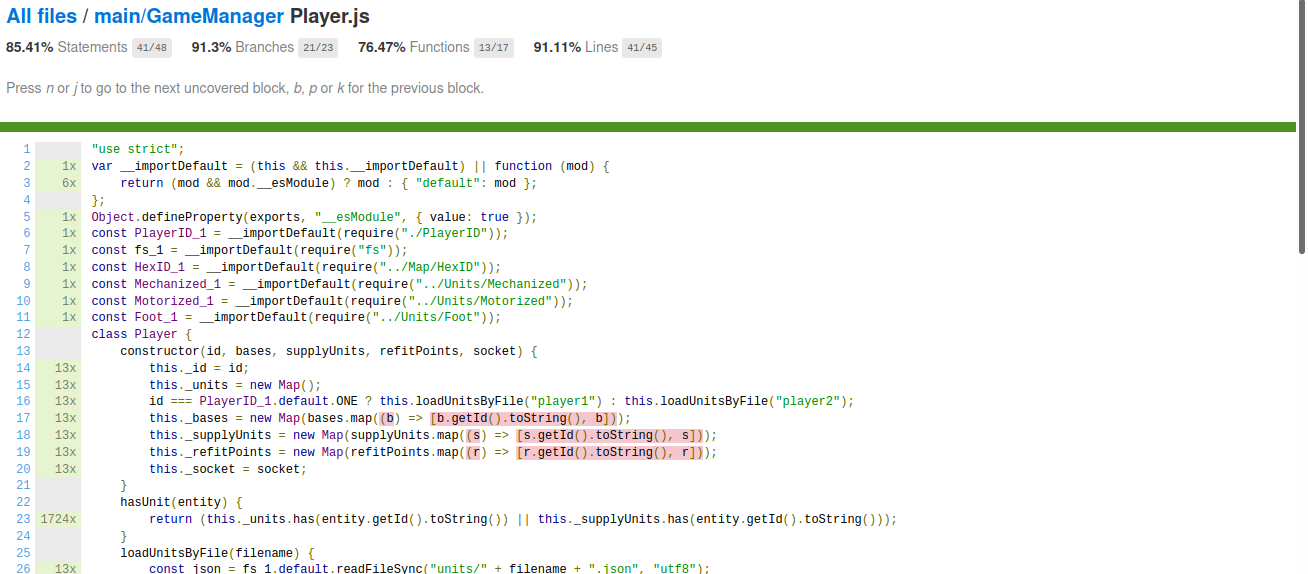
\includegraphics[scale=0.3]{data/couverture_test_2.png}
    \caption{Couverture d'un fichier}
\end{figure}

La couverture du code n'implique pas des tests de qualité. Après quelques recherches, nous avons trouvé qu'une couverture minimale de bonne qualité dépasse les 80\%. Nous nous sommes donc fixés d'au moins atteindre ce pourcentage.